\chapter{Haces con momentum orbital angular (OAM)}

\begin{figure}[H]
	\centering
	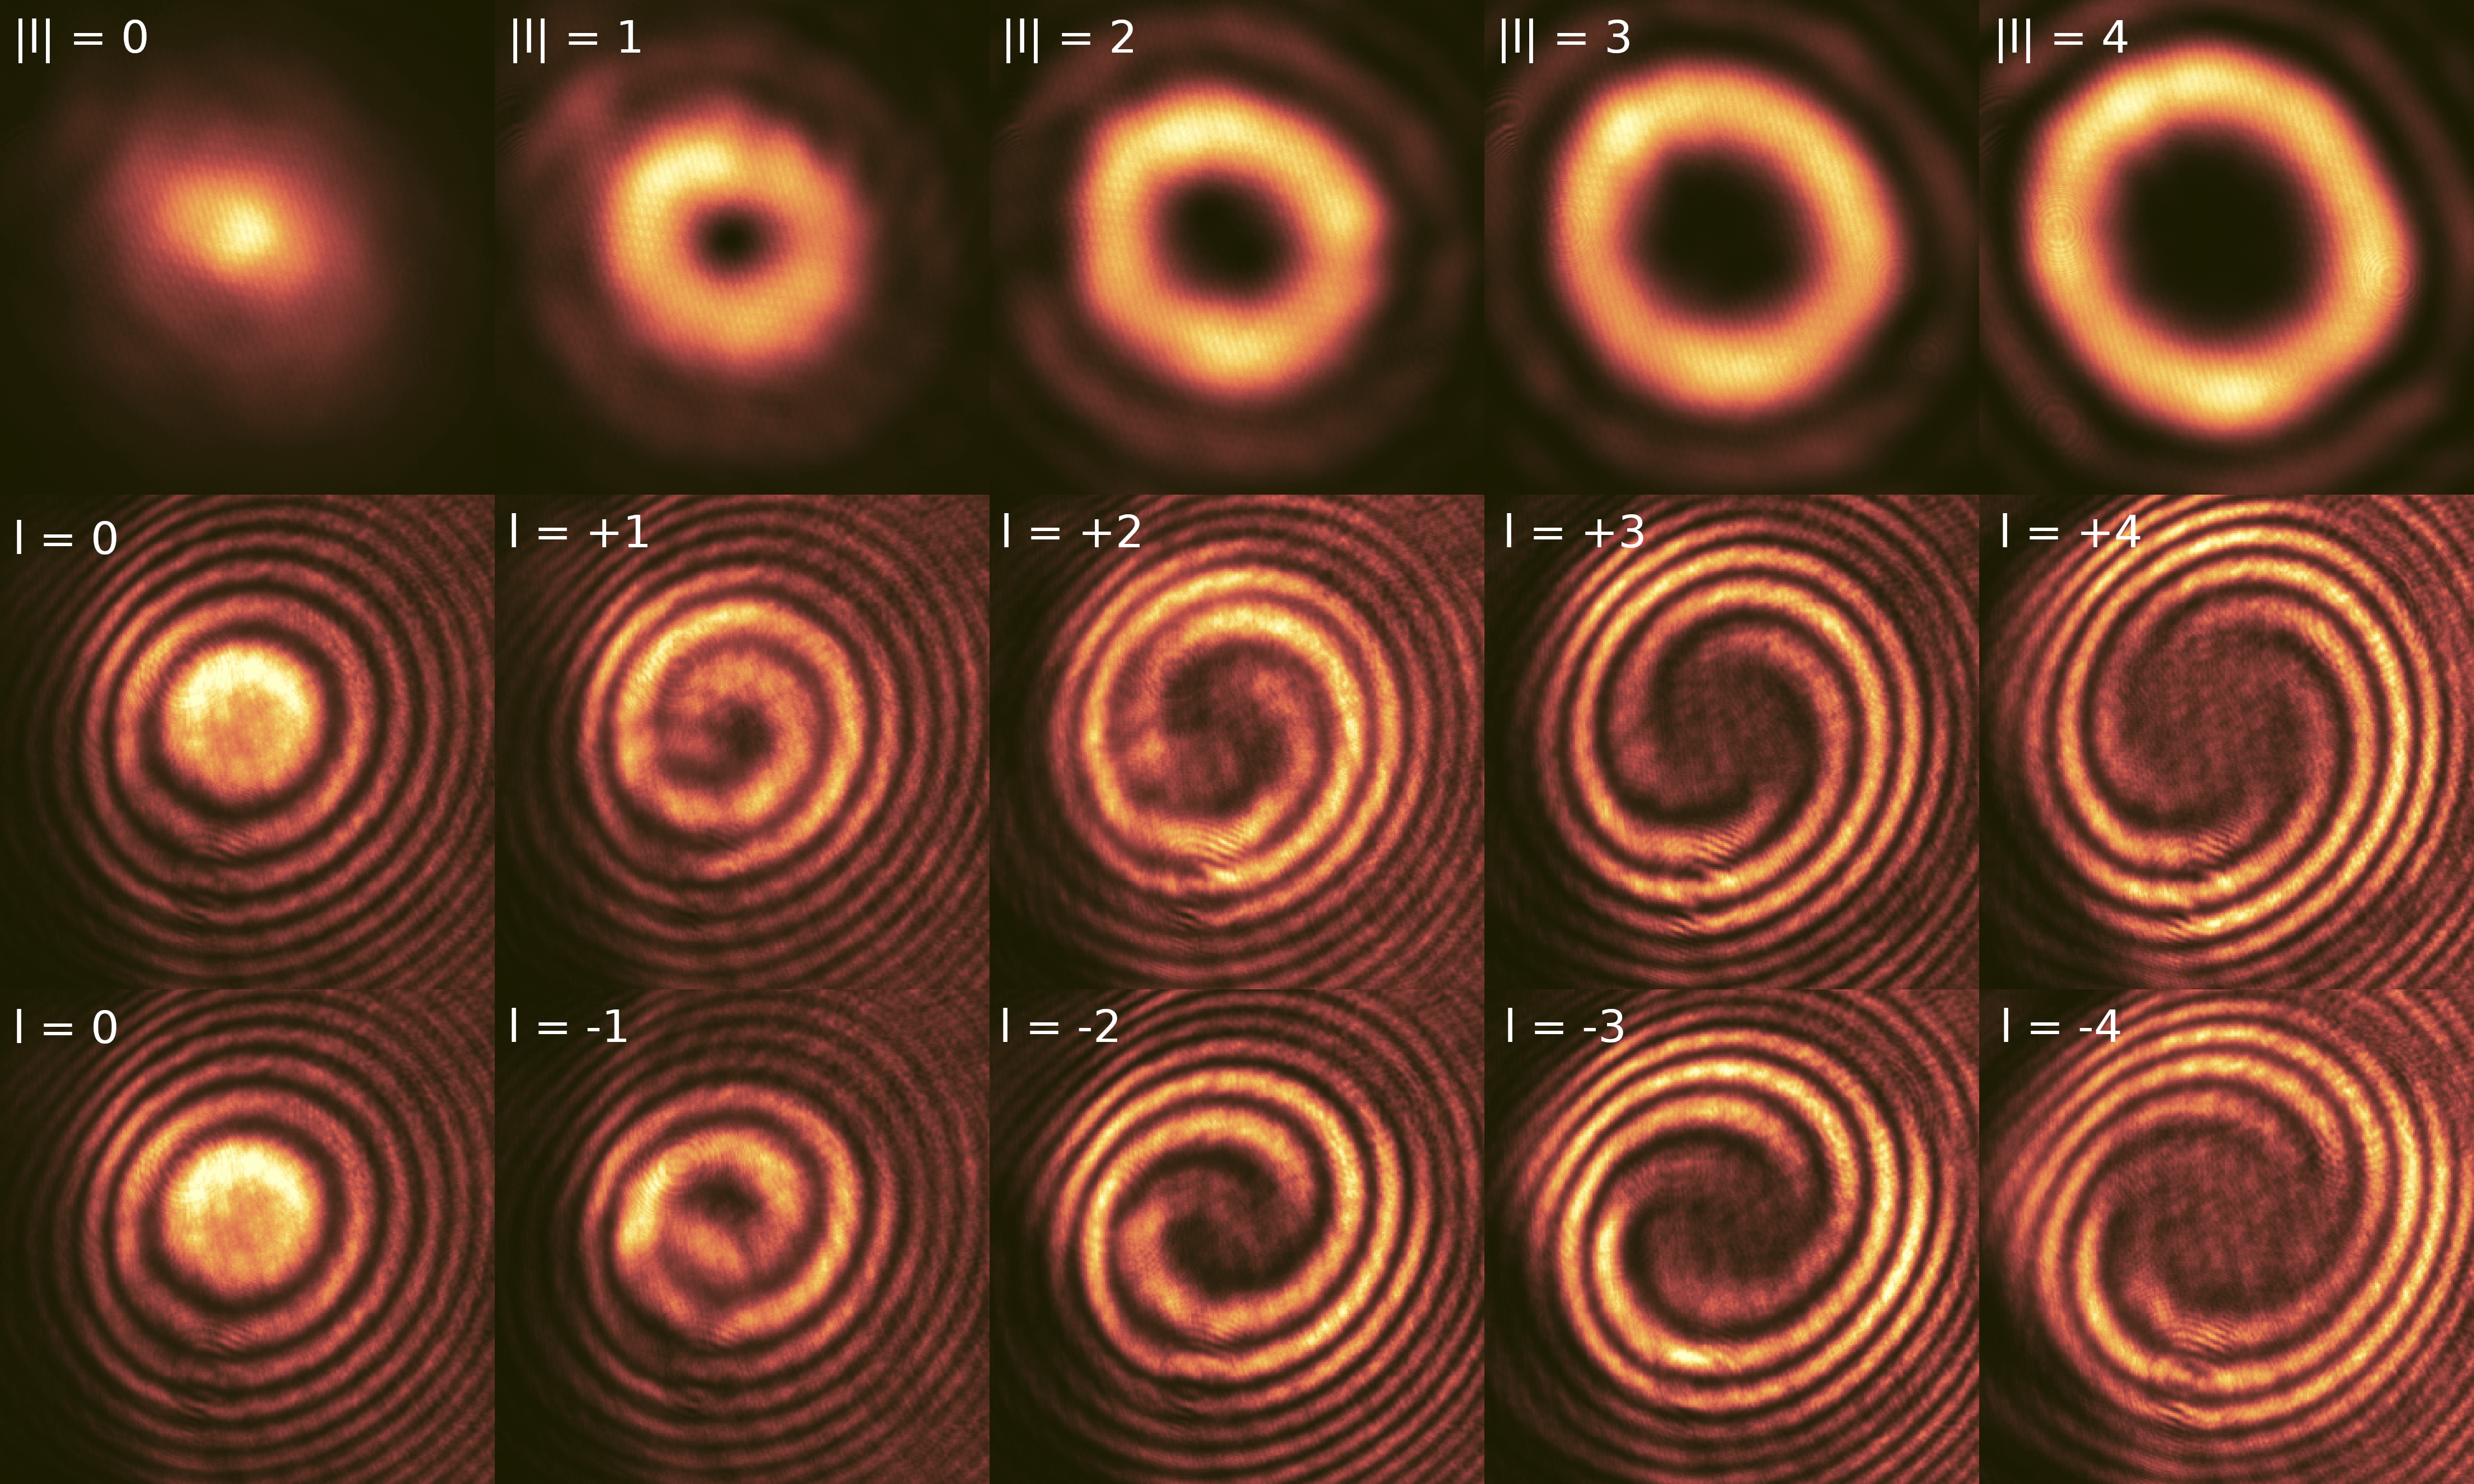
\includegraphics[width=\linewidth]{media/OAM-free.png}
	\caption[Generación de OAMs e interferencia tipo Mach-Zehnder.]{Generación de OAMs e interferencia tipo Mach-Zehnder. Se aprecia la carga de los OAMs contando la cantidad de espirales originados desde el centro.}
\end{figure}